\begin{question}
\noindent Triangle $ABC$ is enlarged to give the image triangle $A'B'C'$, as shown on the grid below.

\begin{center}
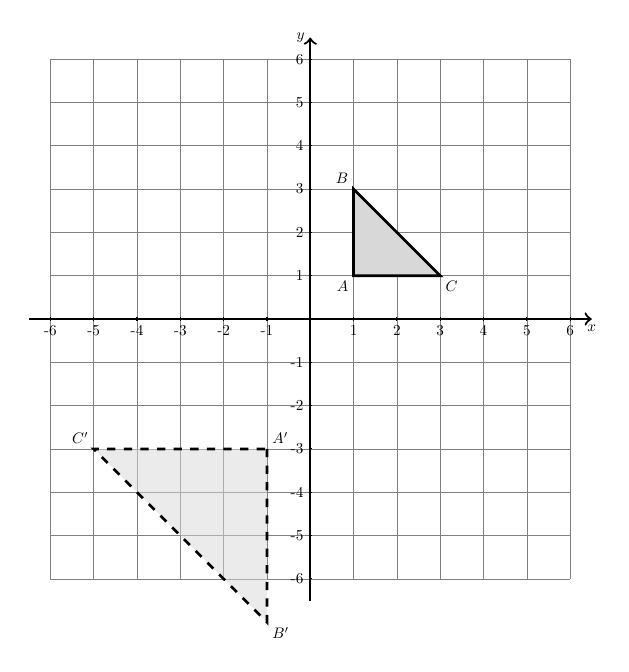
\begin{tikzpicture}[scale=0.55, transform shape]
    \def\axisLimit{6}

    \definecolor{borderColour}{HTML}{000000}
    \definecolor{fillColour}{HTML}{D8D8D8}

    % Draw grid
    \draw[step=1cm,gray,very thin] (-\axisLimit,-\axisLimit) grid (\axisLimit,\axisLimit);

    % Draw axes
    \draw[thick,->] (-\axisLimit-0.5,0) -- (\axisLimit+0.5,0) node[anchor=north] {$x$};
    \draw[thick,->] (0,-\axisLimit-0.5) -- (0,\axisLimit+0.5) node[anchor=east] {$y$};

    % Label x-axis and y-axis
    \foreach \x in {-\axisLimit,...,-1,1,2,...,\axisLimit}
        \draw (\x cm,1pt) -- (\x cm,-1pt) node[anchor=north] {\x};
    \foreach \y in {-\axisLimit,...,-1,1,2,...,\axisLimit}
        \draw (1pt,\y cm) -- (-1pt,\y cm) node[anchor=east] {\y};

    % Original triangle ABC
    \coordinate (A) at (1,1);
    \coordinate (B) at (1,3);
    \coordinate (C) at (3,1);

    \draw[fill=fillColour, draw=borderColour, line width=1pt] (A) -- (B) -- (C) -- cycle;
    \node[below left] at (A) {$A$};
    \node[above left] at (B) {$B$};
    \node[below right] at (C) {$C$};

    % Image triangle A'B'C' (negative enlargement, scale factor -2, centre (1,-1))
    \coordinate (Ap) at (-1,-3);
    \coordinate (Bp) at (-1,-7);
    \coordinate (Cp) at (-5,-3);

    \draw[fill=fillColour, draw=borderColour, line width=1pt, dashed, fill opacity=0.5] (Ap) -- (Bp) -- (Cp) -- cycle;
    \node[above right] at (Ap) {$A'$};
    \node[below right] at (Bp) {$B'$};
    \node[above left] at (Cp) {$C'$};

\end{tikzpicture}
\end{center}

\noindent Triangle $ABC$ has vertices $A(1,1)$, $B(1,3)$ and $C(3,1)$.\\
Triangle $A'B'C'$ has vertices $A'(-1,-3)$, $B'(-1,-7)$ and $C'(-5,-3)$.

\vspace{0.3cm}
\noindent Describe fully the single transformation that maps triangle $ABC$ onto triangle $A'B'C'$.

\vspace{6cm}
\answerlines{3}{4}
\end{question}
